\section{XLNet} \label{sec:XLNet}

While most commonly in NLP models are in the form of neural networks that are pretrained on large, unlabeled data and then fine-tuned for specific tasks, different unsupervised pretraining loss functions have also been explored. From these, \nameref{sec:autoregressiveLM} and \nameref{sec:autoencodingLM} have been the most powerful pretraining objectives. 


\subsection{Problems With BERT}

From Yang et al. (2020), a \emph{forward} \nameref{sec:autoregressiveLM} maximizes the likelihood of an input sequence by using a \emph{forward} autoregressive decomposition, shown in \cref{eq:AutoRegLMLoss}:

\begin{equation}
\textit{max}_\theta \Bigg( \textit{log}  \; P_\theta(\textbf{x})  \Bigg) = \sum_{t=1}^T \textit{log} \; P_\theta \Big(x_t \; | \; \textbf{x}_{< t} \Big)  
\label{eq:AutoRegLMLoss}
\end{equation}


Meanwhile, \nameref{sec:autoencodingLM}s like \nameref{sec:BERT} takes an input sequence $\textbf{x}$, and corrupts it $\hat{\textbf{x}}$ by masking some tokens. The autoencoding model recreates masked tokens $\overline{\textbf{x}}$ from the corrupted input $\hat{\textbf{x}}$, as in \cref{eq:AutoEncodeLMLOSS}:

\begin{equation}
\textit{max}_\theta \Bigg( \textit{log}  \; P_\theta(\overline{\textbf{x}} \; | \; \hat{\textbf{x}})  \Bigg) \;\; \mathlarger{\mathlarger{\approx}} \;\; \sum_{t=1}^T m_t \; \textit{log} \; P_\theta \Big(x_t \; | \; \hat{\textbf{x}} \Big) 
\label{eq:AutoEncodeLMLOSS}
\end{equation}

where $m_t = 1$ indicates that the input token $x_t$ is masked. With this in mind, Yang et al. (2020) note \nameref{sec:BERT}'s problems as follows: 

%\vspace{-10pt}

\begin{enumerateSpaced}{3pt}
    \item \textbf{Independence Assumption: } the $\approx$ approximation sign in \cref{eq:AutoRegLMLoss} indicates \nameref{sec:BERT} factorizes its joint conditional probability $P_\theta(\overline{\textbf{x}} \; | \; \hat{\textbf{x}})$ assuming that all masked tokens $\overline{\textbf{x}}$ are rebuilt independently of each other, even though texts are rife with long-range dependencies. 
    
    \item \textbf{Data Corruption}: Masking tokens from \nameref{sec:BERT}'s \hyperref[sec:maskedlanguagemodelMLM]{masked language modeling} task do not appear in real data during fine-tuning, and since \nameref{sec:BERT} does this in pre-training, a discrepancy arises between these two stages. 
\end{enumerateSpaced}


Kurita (2019b) gives an example to show how BERT predicts tokens independently. Consider the sentence: ``I went to the \texttt{[MASK]} \texttt{[MASK]} and saw the \texttt{[MASK]} \texttt{[MASK]} \texttt{[MASK]}."  Two ways to fill this are:  ($1$) ``I went to \emph{New York} and saw the \textit{Empire State building}," or ($2$) ``I went to \emph{San Francisco} and saw the \emph{Golden Gate bridge}." But \nameref{sec:BERT} might incorrectly mix things up and predict ``I went to \emph{San Francisco} and saw the \emph{Empire State building}." 

Clearly, since \nameref{sec:BERT} predicts masked tokens simultaneously, it fails to learn tokens' interlocking dependencies, which is a major point against \nameref{sec:BERT} since even simple \hyperref[sec:LanguageModels]{language models} learn at least unidirectional token dependencies (Kurita, 2019b). 




\subsection{Motivation for XLNet}

Confronted with \nameref{sec:BERT}'s limitations, Yang et al. (2020) conceived \textbf{XLNet} to keep the benefits of \emph{both} \hyperref[sec:autoencodingLM]{autoencoding} and \hyperref[sec:autoregressiveLM]{autoregressive} language modeling while avoiding their issue. Firstly, the \nameref{sec:autoregressiveLM} objective in XLNet lets the probability $P_\theta(\textbf{x))}$ (from \cref{eq:AutoRegLMLoss}) be factored using the universally-true probability product rule, side-stepping \nameref{sec:BERT}'s false independence assumption. Intuitively this means XLNet can predict tokens sequentially and autoregressively rather than simultaneously like \nameref{sec:BERT}. Secondly, XLNet's \textbf{\hyperref[sec:permutationLM]{permutation language model}} captures bidirectional context like an \hyperref[sec:autoencodingLM]{autoencoding model}. It uses a built-in \hyperref[sec:TwoStreamSelfAttention]{two-stream attention mechanism} to create target-aware predictions. 
 

\subsection{Describing XLNet}


\subsubsection{Permutation Language Model} \label{sec:permutationLM}

Can a model be trained to use \textbf{bidirectional context} while avoiding masking and its resulting problem of independent predictions? Like  \hyperref[sec:LanguageModels]{language model}s, a \textbf{permutation language model} predicts unidirectionally, but instead of predicting in order, the model predicts tokens in a random order. Simply put, a permutation language model must accumulate bidirectional context by finding dependencies between all possible input combinations (Yang et al., 2020). 

Consider the sentence: ``I like cats more than dogs." A traditional \hyperref[sec:LanguageModels]{language model} predicts individual words sequentially from previous context words. But a permutation language model randomly samples prediction order, such as: ``cats", ``than", ``I", ``more", ``dogs", ``like", where ``than" could be conditioned on ``cats" and ``I" might be conditioned on seeing ``cats, than", and so on (Kurita, 2019b). 



%\textbf{NOTE: } the permutation language model only permutes factorization order; it does not change word order in the input sequence, only the order in which words are predicted. XLNet still builds ``target-aware" predictions: input tokens can be fed in arbitrary order into XLNet using a masking feature in the \nameref{sec:Transformer}'s \hyperref[sec:AttentionMechanism]{attention} to temporarily cover certain tokens. Coupled with the use of \hyperref[sec:PosEncodings]{positional embeddings} and their associated original sequences, XLNet will still receive the tokens in correct order (Kurita, 2019b). This improves upon previous versions of permutation models which used an ``implicit position awareness" (Yang et al., 2020). 



\subsubsection{Need for Target-Aware Representations}\label{sec:TargetAwarePred}

Trying to merge \hyperref[sec:permutationLM]{permutation language model} and \nameref{sec:Transformer} blinded XLNet's target predictions to the permutation positions generated by the permutation language model. 

The fault lies in the nature of \nameref{sec:Transformer}s: while predicting a token at a position, \nameref{sec:Transformer} masks the token's embedding but \emph{unfortunately, also} its \hyperref[sec:PosEncodings]{positional encoding}, so it cannot see the position of the target it must predict. Intuitively, this means a sentence cannot be accurately represented, since positions like the beginning of a sentence have different distributions from other positions in the sentence. 

Formally, let $\mathcal{Z}_T =$ all possible permutations of the $T$-length sequence $\Big[1,2,...,T\Big]$; $\;\;\; z_t =$ the $t$-th element and $\textbf{z}_{< t} =$ the vector of the first $t-1$ elements of a permutation $\textbf{z} \in \mathcal{Z}_T$; $\;\;\; \textbf{x} =$ a text sequence of length $T$; $\;\;\; x_{z_t} =$ the content token to be predicted in the text sequence $\textbf{x}_{\textbf{z}_t}$ that is indexed by the permutations in $\textbf{z}_{< t}$. 

Yang et al. (2020) began by parameterizing the next-token predictive distribution using the softmax: 

\begin{equation}
P_\theta \Big( X_{z_t} = x_i\; | \; \textbf{x}_{\textbf{z}_t} \Big) = \frac{\exp {\Big( e(x_i)^T \cdot h_\theta \Big( \textbf{x}_{\textbf{z}_{< t}} \Big) \Big)}}  {\sum_{i=1} \exp{\Big( e(x_i)^T \cdot h_\theta \Big( \textbf{x}_{\textbf{z}_{< t}} \Big) \Big)}}
\label{eq:predDistNoTargetAware}
\end{equation}

where $e(x_i) =$ the embedding of the $i$-th token, $x_i$, and $h_\theta \Big( \textbf{x}_{\textbf{z}_{< t}} \Big) =$ the hidden state vector for $\textbf{x}_{\textbf{z}_t}$ created by the Transformer after masking. But $h_\theta \Big( \textbf{x}_{\textbf{z}_{< t}} \Big)$ does not depend on the position $z_t$ of the target it must predict, so XLNet is limited to predicting the same distribution regardless of target position. To remedy this, the authors replaced the hidden state $h_\theta$ in \cref{eq:predDistNoTargetAware} by $g_\theta \Big( \textbf{x}_{\textbf{z}_{< t}}, \; z_t \Big)$ which takes the target position $z_t$ as an argument. 




\subsubsection{Two-Stream Self-Attention }\label{sec:TwoStreamSelfAttention}

When formulating $g_\theta \Big( \textbf{x}_{\textbf{z}_{< t}}, \; z_t \Big)$ the \nameref{sec:Transformer} architecture produced yet another contradiction: ($1$) to predict token $x_{z_t}$, $g_\theta \Big( \textbf{x}_{\textbf{z}_{< t}}, \; z_t \Big)$ needs only the \emph{position} $z_t$ and not the \emph{content} $x_{z_t}$, or else the prediction becomes trivial, and ($2$) to predict all other tokens $x_{z_j}$ with $j > t$,  $g_\theta \Big( \textbf{x}_{\textbf{z}_{< t}}, \; z_t \Big)$ also needs $x_{z_t}$ to incorporate the entire contextual information. Thus, Dai et al. (2019) invented the \textbf{two-stream attention mechanism} which creates an overall hidden state from two separate sets of hidden states: the \textbf{content stream} and \textbf{query stream}.


The \textbf{content stream} $h_\theta \Big( \textbf{x}_{\textbf{z}_{\leq t}} \Big)$ encodes \emph{context} $\textbf{x}_{\textbf{z} \leq t}$ like ordinary hidden states in the \nameref{sec:Transformer}, while also encoding the \emph{content} token $x_{z_t}$. For the $t$-th prediction in the sentence, the content stream (using both $z_t$ and $x_{z_t}$) is computed for attention layers $m = 1, ..., M$ as $h_{z_t}^{(m)} = \texttt{Attention} \Big( \textbf{Q} = h_{z_t}^{(m-1)}, \;\; \textbf{KV} = \textbf{h}_{ {\color{cyan} \mathlarger{\mathlarger{\mathbf{z}_{\leq t}}}  } }^{(m-1)}; \;\; \theta  \Big)$.

% \begin{codeEnv}{python}
%     # Create permutation sequence: $\mathcal{Z}_T$
%     permutation = permute(range(T))
%     # Initialize content stream attention
%     h = [embeddings] + [Tensor(T) for _ in attentionLayers]
%     
%     for m, attention in enumerate(attentionLayers):
%         for t, position in enumerate(permutation):
%             # Including the current word (t) in the visible positions because of the $\textbf{h}_{ {\color{IndianRed} \mathlarger{\mathlarger{\mathbf{z}_{\leq t}}}  } }^{(m-1)}$
%             visiblePositions = permutation[:t+1]
%             # Content stream formula
%             h[m][position] = attention(queries = q[m-1][position], keys = h[m-1][visiblePositions], values = h[m-1][visiblePositions])
%     
% \end{codeEnv}
% \vspace{-20pt}
% \captionof{listing}{Content stream calculation}
% \label{code:ContentStreamAttn}
% \setlength{\parskip}{5pt}


\textbf{Query stream} $g_\theta \Big( \textbf{x}_{\textbf{z}_{< t}}, \; z_t \Big)$ encodes \emph{context} $\textbf{x}_{\textbf{z} \leq t}$ with \emph{position} $z_t$ simultaneously, but not the \emph{content} token $x_{z_t}$, to evade the contradiction. For the $t$-th prediction in a sentence, the query stream (using $z_t$ but not $x_{z_t}$) is computed as $g_{z_t}^{(m)} = \texttt{Attention} \Big( \textbf{Q} = g_{z_t}^{(m-1)}, \;\; \textbf{KV} = \textbf{h}_{ {\color{cyan} \mathlarger{\mathlarger{\mathbf{z}_{< t}}}  } }^{(m-1)}; \;\; \theta  \Big)$.


% \begin{codeEnv}{python}
%     # Create permutation sequence: $\mathcal{Z}_T$
%     permutation = permute(range(T))
%     # Compute the content stream as in above listing:
%     contentStrm = computeContentStream(permutation)
%     # Initialize query stream
%     q = [w] + [Tensor(T) for _ in attentionLayers]
%     
%     for m, attention in enumerate(attentionLayers):
%         for t, position in enumerate(permutation):
%             # Excluding the current word (t) in the visible positions because of the $\textbf{h}_{ {\color{IndianRed} \mathlarger{\mathlarger{\mathbf{z}_{< t}}}  } }^{(m-1)}$
%             visiblePositions = permutation[:t]
%             # Query stream formula
%             q[m][position] = attention(queries = q[m-1][position], keys = contentStrm[m-1][visiblePositions], values = contentStrm[m-1][visiblePositions])
%     
% \end{codeEnv}
% \vspace{-20pt}
% \captionof{listing}{Query stream calculation}
% \label{code:QueryStreamAttn}
% \setlength{\parskip}{5pt}
% %TODO: adding manual restoration of parskip here because it gets removed after the codesnippet - why? 


Intuitively, the purpose of the content and query stream is as follows. Suppose we must predict the word ``like" in \textit{``I like cats more than dogs"} where the previous words in the permutation were ``more" and ``dogs." The \textbf{content stream} would encode this information while the \textbf{query stream} would hold positional knowledge about ``like" as well as content stream information, so XLNet can predict ``like" (Kurita, 2019b). 



%\subsubsection{Using Transformer-XL}

%XLNet uses the \hyperref[sec:SegmentLevelRec]{segment-level recurrence mechanism} and \hyperref[sec:RelativePosEnc]{relative encodings}


\subsubsection{Relative Segment Encodings}\label{sec:RelativeSegmentEncodings}

XLNet builds on \nameref{sec:TransformerXL}'s \hyperref[sec:RelativePosEnc]{relative encodings} to model relationships between positions. While \nameref{sec:BERT} learns a segment embedding to distinguish \emph{which specific segments the (words) positions are from}, XLNet learns an embedding that encodes if two words are \emph{within the same segment embedding}. As a benefit, XLNet can be applied to tasks that take arbitrarily many input sequences (Kurita, 2019b).


\subsection{Conceptual Difference Between XLNet and BERT}
%\subsection{Experimental Results of XLNet}

To further illustrate the conceptual difference between XLNet and \nameref{sec:BERT} from a model training standpoint, take the list of words $\Big[ \texttt{New}, \texttt{York}, \texttt{is}, \texttt{a}, \texttt{city} \Big]$. Let the two tokens $\Big[ \texttt{New}, \texttt{York} \Big]$ be selected for prediction, so the models must maximize the log-likelihood: $\text{log} \; P(\texttt{New York} \; | \; \texttt{is a city})$. Assuming XLNet uses the factorization order $\Big[ \texttt{is}, \texttt{a}, \texttt{city}, \texttt{New}, \texttt{York} \Big]$, then \nameref{sec:BERT} and XLNet have the following loss functions: 

\begin{equation}
\begin{array}{ll}
\mathcal{J}_\text{BERT} = \text{log} \; P \Big( \texttt{New} \; | \; \texttt{is a city} \Big) \; + \; \text{log} \; P \Big( \texttt{York} \; | \; \texttt{is a city} \Big) \\
\mathcal{J}_\text{XLNet} = \text{log} \; P \Big( \texttt{New} \; | \; \texttt{is a city} \Big) \; + \; \text{log} \; P \Big( \texttt{York} \; | \; {\color{cyan} \texttt{New}}, \texttt{is a city} \Big) 
\end{array}
\label{eq:XLnetVsBERTLogLiks}
\end{equation}


While \nameref{sec:BERT} can learn some kind of dependency between the pairs \texttt{New} and \texttt{York}, \cref{eq:XLnetVsBERTLogLiks} clearly shows that XLNet learns stronger dependency or a ``denser training signal" (Dai et al., 2019). 

%For reading comprehension datasets like SQuAD and RACE where longer-context representation is required, XLNet outperformed \nameref{sec:BERT} as measured by their GLUE scores in \cref{tbl:xlnet_generalResults}.


% \begin{figure}[h]
% \vspace{-5pt}
% \centering
% 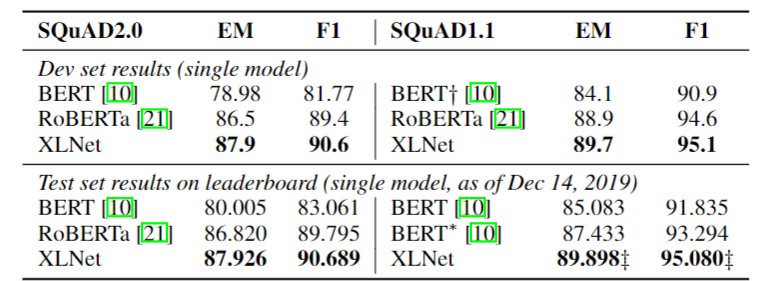
\includegraphics[width=0.7\textwidth]{imgs/xlnet_tableGeneralResults.png}
% \vspace{-5pt}
% \captionof{table}{\footnotesize Comparing GLUE scores of \nameref{sec:BERT} and BERT-based model called RoBERTa with XLNet. From \emph{Table 3 in XLNet: Generalized Autoregressive Pretraining for Language Understanding}, by Dai et al., 2019. \url{https://arxiv.org/pdf/1906.08237.pdf}. Copyright 2019 by Dai et al.}
% \vspace{-5pt}
% \label{tbl:xlnet_generalResults}
% \end{figure}


%Dai et al. (2019) used an ablation study to determine which component of XLNet is better than \nameref{sec:BERT}:  the \hyperref[sec:permutationLM]{permutation language model}, the \nameref{sec:TransformerXL} backbone, or some other details used in implementation, such as span-based prediction and next sentence prediction. The \cref{tbl:xlnet_ablationStudy} compares \nameref{sec:BERT}, \nameref{sec:TransformerXL}, and XLNet variations. Rows 1-4 show that \nameref{sec:TransformerXL} and the \hyperref[sec:permutationLM]{permutation language model} contribute to XLNet's success since its scores across different datasets are higher than for \nameref{sec:BERT}. Row 5 shows removing the memory caching reduces performance for the longer-context containing RACE data set. 

% 
% \begin{figure}[h]
% \vspace{-5pt}
% \centering
% 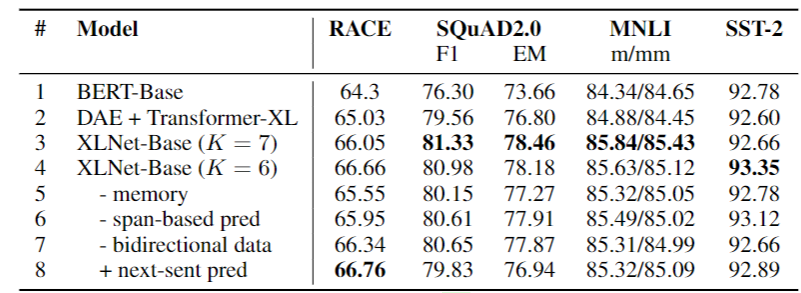
\includegraphics[width=0.7\textwidth]{imgs/xlnet_tableAblation.png}
% \vspace{-5pt}
% \captionof{table}{\footnotesize Ablation study for XLNet's \hyperref[sec:permutationLM]{permutation language model} on RACE, SQuAD, MNLI, SST-2 datasets. From \emph{Table 6 in XLNet: Generalized Autoregressive Pretraining for Language Understanding}, by Dai et al., 2019. \url{https://arxiv.org/pdf/1906.08237.pdf}. Copyright 2019 by Dai et al.}
% \vspace{-5pt}
% \label{tbl:xlnet_ablationStudy}
% \end{figure}
% 


%XLNet's integration of an \nameref{sec:autoregressiveLM} with \nameref{sec:TransformerXL} and a \hyperref[sec:TwoStreamSelfAttention]{two-stream attention mechanism} results in clear improvements over \hyperref[sec:maskedlanguagemodelMLM]{masked language models} like \nameref{sec:BERT}, which are prone to false assumptions and data corruption. 